% ====================================================================
%  Chapter: Multi-Agent AI Pipeline Architecture
% ====================================================================
\newpage
\section{Multi-Agent AI Pipeline Architecture}
\label{sec:multi-agent}

This section presents the conversational intelligence architecture of H.E.R.A. The current implementation is not a single chatbot placed in front of the IoT system. Instead, it is a graph-based multi-agent runtime that separates routing, device planning, telemetry reporting, anomaly analysis, web research, memory handling, policy checking, and final response composition. This separation is important because H.E.R.A must both communicate naturally with users and safely control physical devices. A natural-language error in a casual response is tolerable; an incorrect actuator command is not. Therefore, the architecture is designed around explicit contracts, bounded tool capabilities, deterministic guards, and auditable execution results.

\subsection{Design Gap and Architectural Motivation}

The core technical gap addressed by this architecture is the mismatch between open-ended language generation and safety-critical IoT control. Large language models are effective at interpreting natural language, but they are probabilistic systems. If an LLM is allowed to directly generate MQTT commands or directly decide whether an environmental condition is dangerous, the system becomes difficult to verify. In a smart-home context, this creates three risks:

\begin{itemize}[leftmargin=*, itemsep=2pt]
    \item \textbf{Tool ambiguity:} user phrases such as ``turn it off'' or ``make the room darker'' require grounding to a concrete device, property, and value.
    \item \textbf{State inconsistency:} an LLM may claim a device was controlled even when the hardware is offline or already in the requested state.
    \item \textbf{Evaluation difficulty:} if routing, reasoning, tool execution, and response generation are mixed in one prompt, failures cannot be attributed to a specific layer.
\end{itemize}

H.E.R.A addresses this gap using an orchestrator-specialist architecture implemented as a LangGraph state machine. The LLM is used where semantic interpretation is valuable, while deterministic software is used for policy, validation, telemetry freshness, anomaly classification, and execution verification. This division is the central design principle of the AI subsystem.

\subsection{Current H.E.R.A AI Architecture}

Figure~\ref{fig:hera-ai-overall-architecture} shows the current conversational intelligence core of H.E.R.A. This diagram focuses only on the AI layer, not the full hardware, database, or frontend architecture of the whole system. The user request first enters the request-understanding stage, where the input is normalized and prepared as a structured message. It is then passed to the H.E.R.A orchestrator, which coordinates routing, memory access, specialist selection, runtime tool execution, and final response generation. Supporting systems such as memory, specialist modules, safety verification, and the tool system are shown as indirect dependencies because they do not replace the main request path; instead, they provide context, capabilities, and validation to the core pipeline. \\

The high-level flow can be read from left to right. A natural-language request becomes a normalized request, the orchestrator decides how it should be handled, a specialist produces either a domain report or a tool-oriented plan, the runtime tool boundary validates and executes the required tool calls, and the response generator converts the verified result into a user-facing answer. This separation is important because it keeps language interpretation, tool execution, and final explanation as distinct stages. In particular, the LLM does not directly publish MQTT commands. It can only propose structured actions that must pass through the runtime boundary.

\begin{figure}[H]
    \centering
    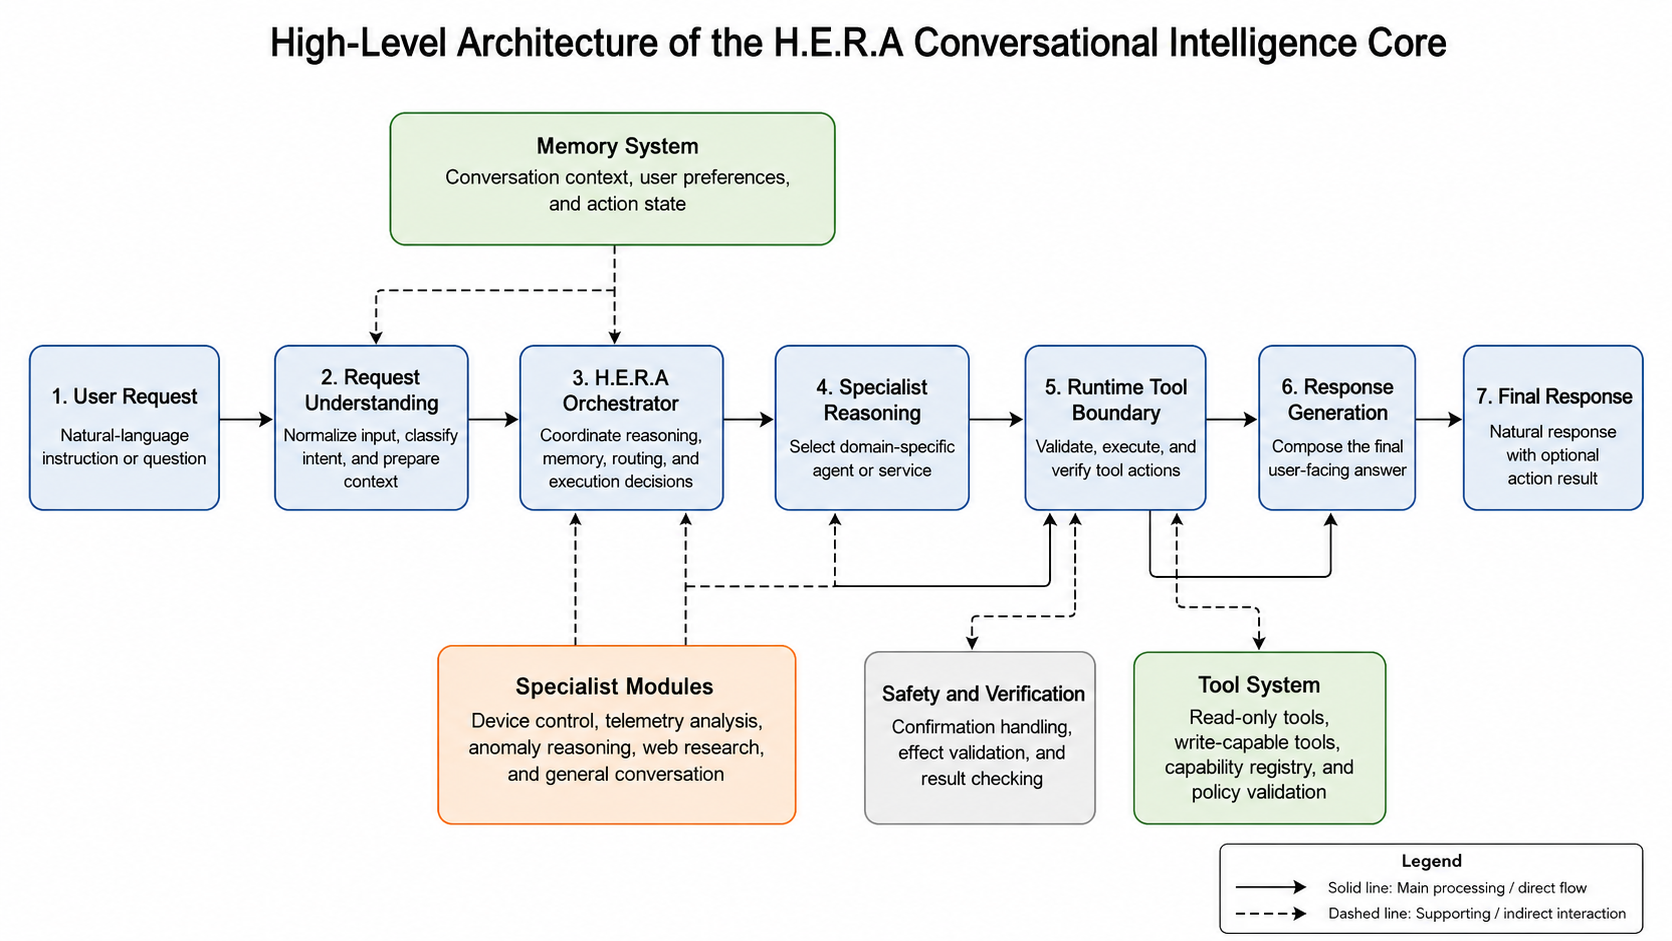
\includegraphics[width=0.98\textwidth]{image/system/high_level_architecture.png}
    \caption{Current layered architecture of the H.E.R.A multi-agent AI subsystem.}
    \label{fig:hera-ai-overall-architecture}
\end{figure}

Figure~\ref{fig:hera-orchestrator-block} expands the orchestration block shown in the high-level architecture. The orchestrator acts as the decision center between the user-facing API and the specialist/runtime layers. It first performs request-state intake, routes the message by intent, checks pending confirmation state, and selects the memory context required for the current request. The routing result then determines whether the request can be handled as general conversation, dispatched to a specialist, or sent into the tool-calling path. Only after this state gate does the system enter the runtime execution block. The final response is composed from the specialist report and any verified runtime result, rather than from unconfirmed model text alone.

\begin{figure}[H]
    \centering
    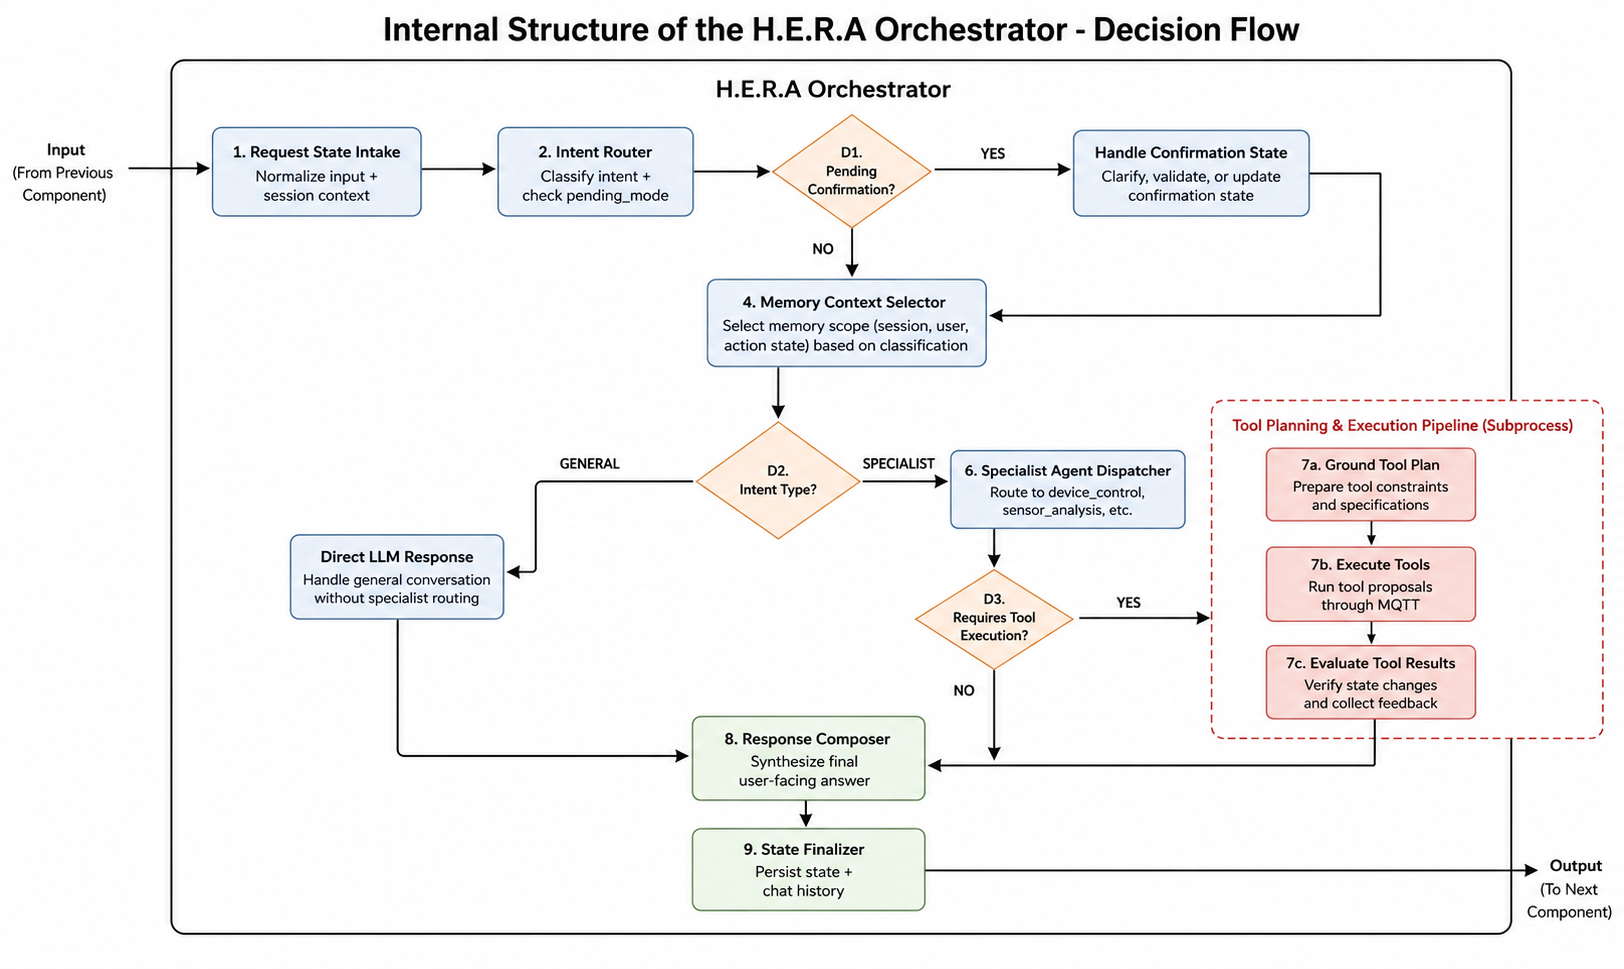
\includegraphics[width=0.98\textwidth]{image/system/orchestrator_block.png}
    \caption{Detailed orchestrator pipeline block inside the H.E.R.A multi-agent AI subsystem.}
    \label{fig:hera-orchestrator-block}
\end{figure}

The red subprocess in Figure~\ref{fig:hera-orchestrator-block} represents the tool-calling and runtime execution block. This block is expanded in Figure~\ref{fig:hera-tool-calling-block}. Its input is a set of grounded tool calls or capability proposals produced by the specialist path. Its output is a normalized tool-execution result that returns to the response composer. Between those two points, the runtime performs capability validation, policy checking, read/write routing, optional confirmation handling, tool execution, result normalization, and effect verification. \\

The read-only path is used for operations such as retrieving current telemetry, device status, or recent telemetry windows. These operations do not mutate external device state and can therefore be executed through a simpler read-tool runner. The write-capable path is stricter. It checks whether the target and arguments are valid, whether policy allows the action, whether user confirmation is required, and whether the physical effect can be verified after execution. This design keeps tool calling auditable: every runtime result has an explicit status, policy decision, and verification fact that can be used by the response composer and later evaluation logs.

\begin{figure}[H]
    \centering
    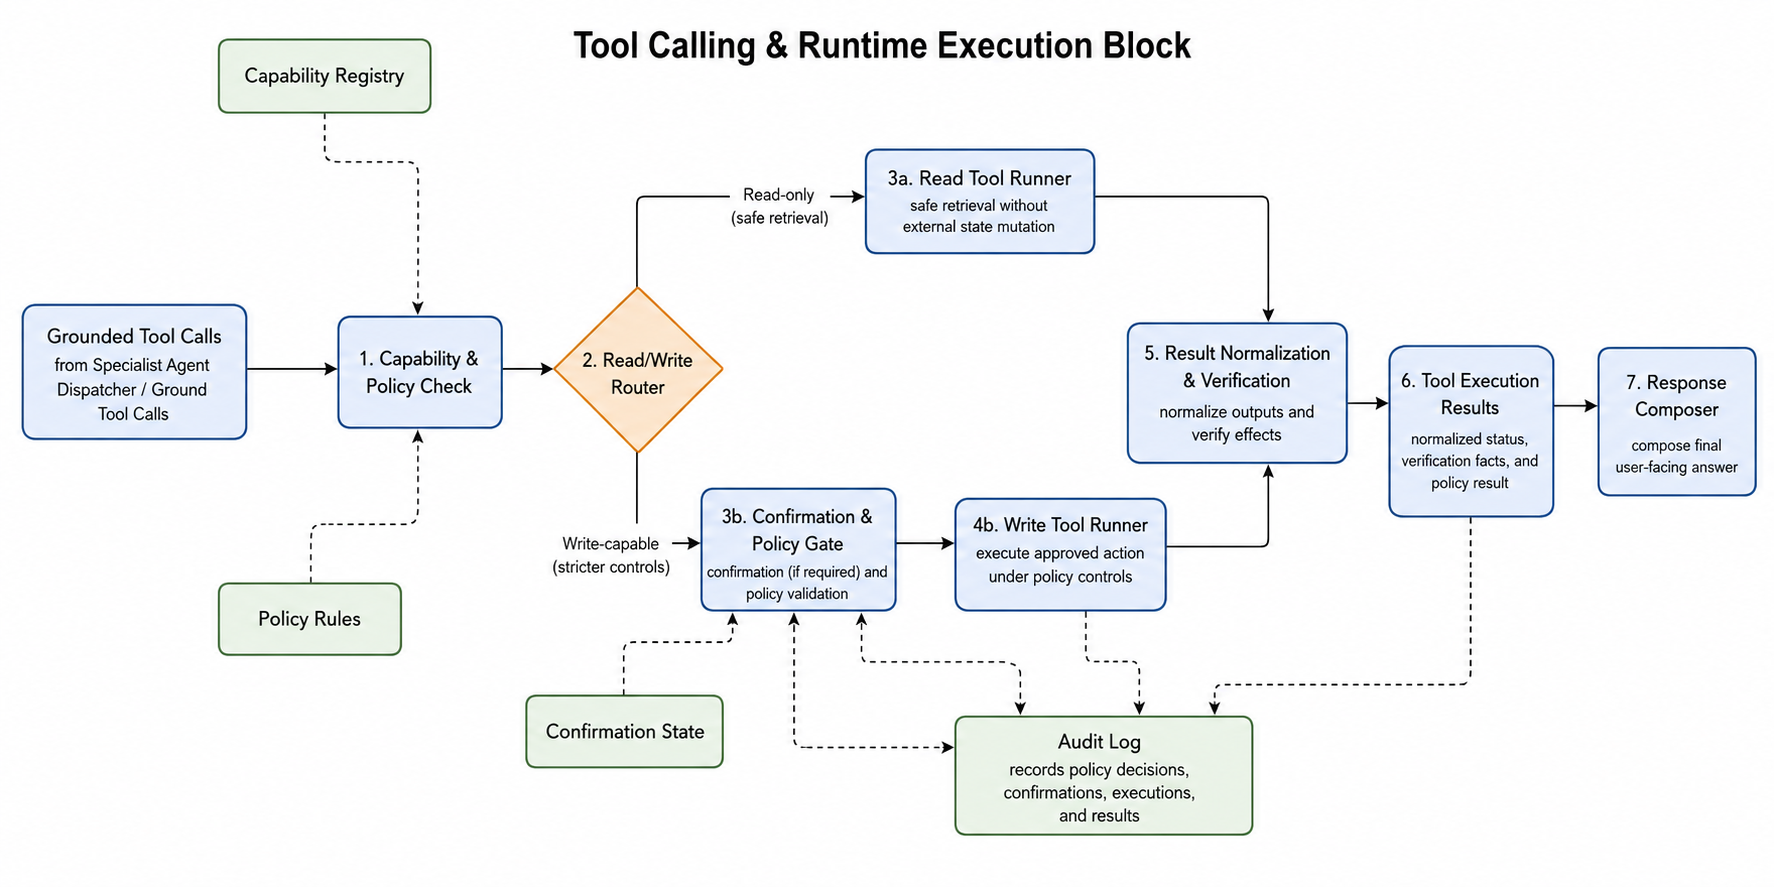
\includegraphics[width=0.98\textwidth]{image/system/tool_block.png}
    \caption{Internal flow of the H.E.R.A tool-calling and runtime execution block.}
    \label{fig:hera-tool-calling-block}
\end{figure}

Together, Figures~\ref{fig:hera-ai-overall-architecture}, \ref{fig:hera-orchestrator-block}, and \ref{fig:hera-tool-calling-block} describe the same request flow at three levels of detail. The first figure shows where the AI core sits conceptually, the second figure shows how the orchestrator chooses the processing route, and the third figure shows how concrete tool calls are validated and executed. This layered presentation reflects the implementation principle of H.E.R.A: the AI system may interpret and plan, but physical effects must pass through deterministic runtime boundaries before they are reported back to the user.

The architecture contains five main functional layers:

\begin{table}[H]
    \centering
    \caption{Functional layers of the H.E.R.A AI subsystem}
    \label{tab:hera-ai-layers}
    \renewcommand{\arraystretch}{1.2}
    \begin{tabularx}{\textwidth}{@{}p{3.1cm}X@{}}
        \toprule
        \textbf{Layer} & \textbf{Responsibility} \\
        \midrule
        Interface layer & Receives user input from REST/dashboard or other adapters and converts it into a unified \texttt{UserMessage}. \\
        Orchestration layer & Classifies intent, selects memory scope, handles pending confirmations, routes to specialists, and composes the final user-facing response. \\
        Specialist layer & Performs domain-specific planning or reporting: device control, telemetry reporting, anomaly analysis, and web research. \\
        Runtime layer & Converts plans into capability proposals, checks policy, executes read/write tools, verifies effects, and records structured results. \\
        Infrastructure layer & Provides LLM inference, MQTT communication, MongoDB memory/telemetry storage, and external search services. \\
        \bottomrule
    \end{tabularx}
\end{table}

\subsection{LangGraph Execution Model}

The current H.E.R.A orchestrator is implemented as a LangGraph state machine rather than a simple sequential function. The graph is compiled with an in-memory checkpointer keyed by the user session, allowing the runtime to preserve thread state such as chat history, active device focus, pending confirmation, pending device clarification, and previous tool results. Figure~\ref{fig:hera-langgraph-flow} summarizes the graph.

\begin{figure}[H]
    \centering
    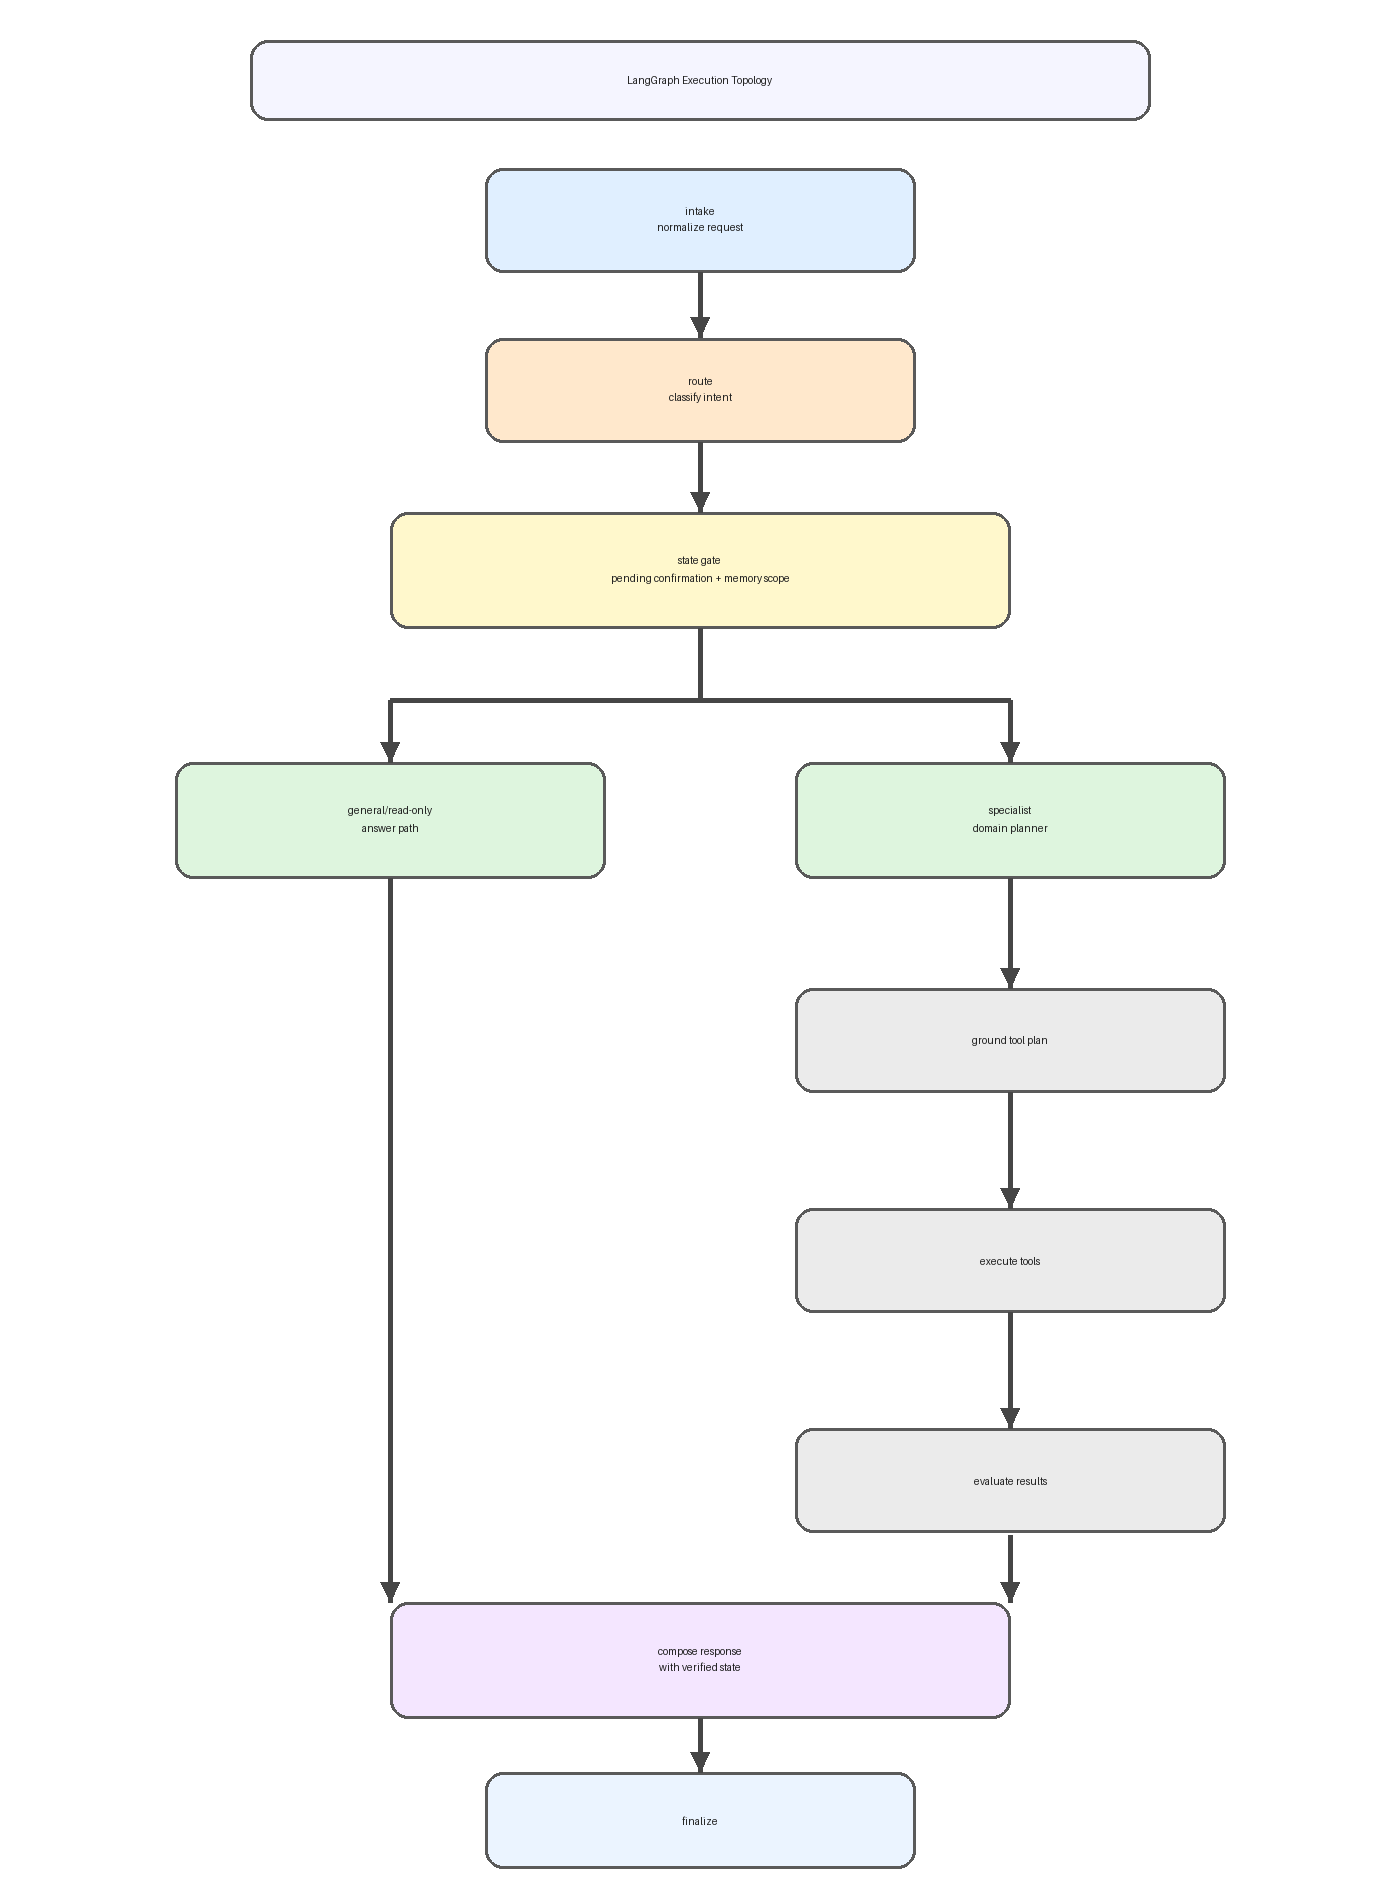
\includegraphics[width=0.82\textwidth]{image/langgraph.png}
    \caption{LangGraph execution topology of the H.E.R.A orchestrator.}
    \label{fig:hera-langgraph-flow}
\end{figure}

The graph separates planning from execution. A specialist does not directly control hardware. It returns a structured report or a set of tool proposals. The runtime tool node then executes those proposals through the central tool runner. This allows policy enforcement and verification to be applied uniformly, whether the request originates from the chat interface or the dashboard.

\subsection{Intent Taxonomy and Routing}

The orchestrator recognizes five intent categories:

\begin{table}[H]
    \centering
    \caption{Intent taxonomy used by the orchestrator}
    \label{tab:hera-intent-taxonomy}
    \renewcommand{\arraystretch}{1.18}
    \begin{tabularx}{\textwidth}{@{}p{3.0cm}p{3.1cm}X@{}}
        \toprule
        \textbf{Intent} & \textbf{Specialist} & \textbf{Purpose} \\
        \midrule
        \texttt{device\_control} & \texttt{device\_control} & Parse actuator requests, generate capability proposals, and route write operations through policy and verification. \\
        \texttt{sensor\_query} & \texttt{telemetry\_report} & Report current temperature, humidity, light, anomaly score, device state, and network state. \\
        \texttt{anomaly\_query} & \texttt{anomaly\_analyzer} & Explain abnormal telemetry based on freshness, thresholds, anomaly score, and recent telemetry windows. \\
        \texttt{web\_search} & \texttt{web\_research} & Retrieve current external information using bounded search/fetch services. \\
        \texttt{general} & \texttt{orchestrator} & Handle greetings, help requests, and non-effectful conversation. \\
        \bottomrule
    \end{tabularx}
\end{table}

The routing prompt returns not only an intent but also a memory policy. The memory scope can be \texttt{none}, \texttt{session}, \texttt{actions}, \texttt{profile}, or \texttt{all}. This distinction prevents unnecessary memory retrieval for simple current-state questions while allowing contextual commands such as ``turn it off'' to use recent actions or active focus. The router also has a safety correction step: if a message is classified as a sensor or general request but the device planner semantically recognizes a valid actuator command, the orchestrator forces the full device-control graph.

\subsection{Short-Path Optimization for Read-Only Requests}

H.E.R.A includes an optimized short path for simple non-effectful requests. If the intent is \texttt{sensor\_query}, \texttt{anomaly\_query}, or trusted \texttt{general}, and the router declares that no memory is needed, the orchestrator can respond without executing the full graph. This is shown in Figure~\ref{fig:hera-shortpath}.

\begin{figure}[H]
    \centering
    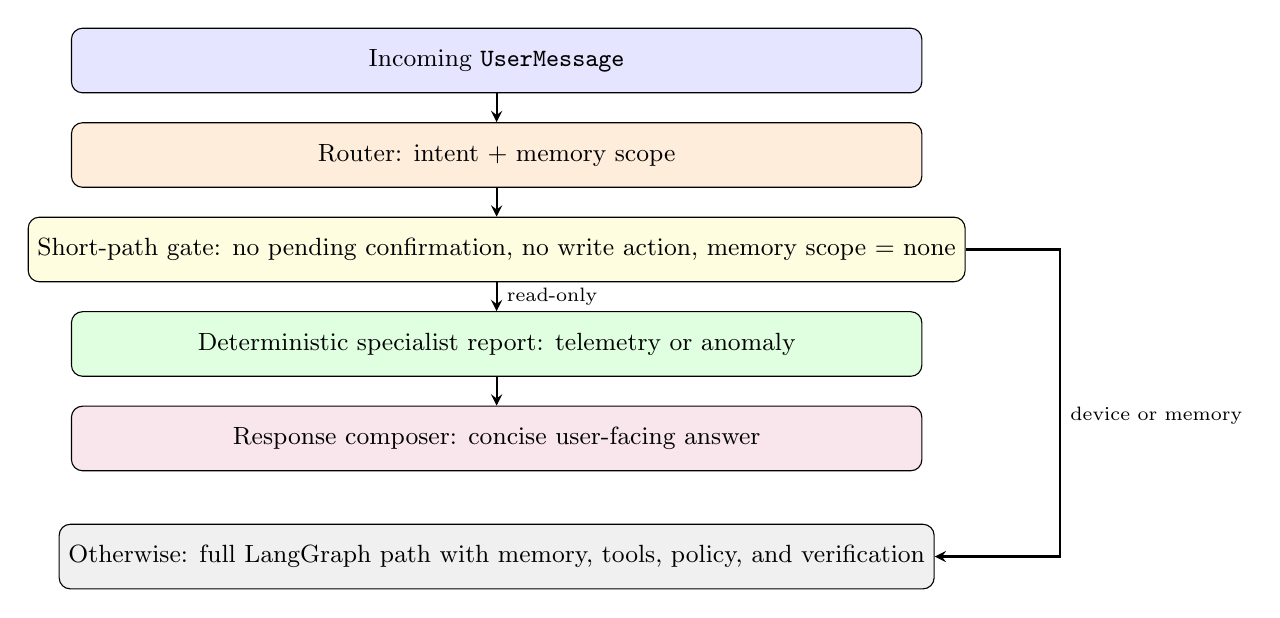
\begin{tikzpicture}[
            box/.style={draw, rounded corners, minimum width=10.8cm,
                    minimum height=0.82cm, align=center, font=\small},
            arrow/.style={->, >=stealth, thick}
        ]
        \node[box, fill=blue!10] (msg) at (0,0) {Incoming \texttt{UserMessage}};
        \node[box, fill=orange!14] (router) at (0,-1.2) {Router: intent + memory scope};
        \node[box, fill=yellow!12] (gate) at (0,-2.4) {Short-path gate: no pending confirmation, no write action, memory scope = none};
        \node[box, fill=green!12] (report) at (0,-3.6) {Deterministic specialist report: telemetry or anomaly};
        \node[box, fill=purple!10] (reply) at (0,-4.8) {Response composer: concise user-facing answer};
        \node[box, fill=gray!12] (full) at (0,-6.3) {Otherwise: full LangGraph path with memory, tools, policy, and verification};

        \draw[arrow] (msg) -- (router);
        \draw[arrow] (router) -- (gate);
        \draw[arrow] (gate) -- node[right, font=\scriptsize] {read-only} (report);
        \draw[arrow] (report) -- (reply);
        \draw[arrow] (gate.east) -- ++(1.2,0) |- node[pos=0.27, right, font=\scriptsize] {device or memory} (full.east);
    \end{tikzpicture}
    \caption{Short-path optimization for read-only AI requests.}
    \label{fig:hera-shortpath}
\end{figure}

This design reduces latency and cost because routine status questions do not require a full agent graph or a tool-execution cycle. More importantly, it preserves safety because device-control requests are explicitly excluded from the short path.

\subsection{Specialist Components}

\subsubsection{Device Control Agent}

The Device Control Agent converts natural language actuator requests into structured capability proposals. It uses the configured device-control model to parse a command into an action, target, optional property, optional value, optional condition, and confidence score. Supported actions include:

\begin{itemize}[leftmargin=*, itemsep=2pt]
    \item \texttt{turn\_on} and \texttt{turn\_off} for binary device control.
    \item \texttt{status} for reading current device state.
    \item \texttt{set\_device\_value} for brightness, color, and fan-speed control.
    \item \texttt{set\_sensor\_value} for simulator-only sensor overrides.
\end{itemize}

The agent grounds natural language targets using a physical placement catalog. This allows the user to speak in room-level terms rather than internal device identifiers. Table~\ref{tab:hera-device-placement-map} shows the current mapping between runtime device targets, physical locations, and user-facing names.

\begin{table}[H]
    \centering
    \caption{Device placement mapping used by the H.E.R.A AI and digital-twin layers}
    \label{tab:hera-device-placement-map}
    \renewcommand{\arraystretch}{1.16}
    \small
    \begin{tabularx}{\textwidth}{@{}p{2.6cm}p{2.8cm}p{2.5cm}X@{}}
        \toprule
        \textbf{Runtime target} & \textbf{User-facing device} & \textbf{Room} & \textbf{Supported control semantics} \\
        \midrule
        \texttt{main\_led} & Living room light & Living Room & On/off control for the main indicator LED. \\
        \texttt{neo\_led} & Bedroom light & Bedroom & On/off control and brightness adjustment for the NeoPixel strip. \\
        \texttt{ws2812} & Toilet light & Toilet & On/off control, brightness adjustment, and RGB color control. \\
        \texttt{mini\_fan} & Living room fan & Living Room & On/off control and fan-speed adjustment. \\
        \texttt{relay} & Living room TV & Living Room & On/off relay control for the TV load. \\
        \texttt{all\_lights} & All lights & Multiple rooms & Group target for all lighting devices. \\
        \texttt{all\_devices} & All devices & Whole house & Broad group target; requires confirmation before execution. \\
        \bottomrule
    \end{tabularx}
\end{table}

The agent also supports conditional commands. For example, a request such as ``turn on the fan if the temperature is above 35 degrees'' is parsed as a device action plus a sensor threshold. The condition is then grounded against the current telemetry snapshot or a telemetry window before any write tool is produced. This prevents the model from executing a conditional command without validating the condition against data.

\subsubsection{Telemetry Report Service}

The Telemetry Report Service is deterministic. It does not ask an LLM to infer current sensor values. Instead, it reads the current MQTT snapshot through the read-tool boundary and returns a structured specialist report. The report includes the current snapshot, data-source metadata, availability flags, and reference thresholds for temperature, humidity, and anomaly score. The final response may be natural-language text, but the facts come from runtime telemetry.

\subsubsection{Anomaly Analyzer Service}

The Anomaly Analyzer Service is also deterministic. It first checks telemetry freshness using the configured stale threshold. If telemetry is stale or missing, the service reports an unknown current-state severity rather than making an unsupported conclusion. If telemetry is fresh, it classifies anomaly status using rule-based checks over temperature, humidity, and anomaly score. It also reads a recent telemetry window from MongoDB when available. The LLM is used only to explain the structured result, not to decide whether an anomaly exists.

\subsubsection{Web Research Service}

The Web Research Service handles external and time-sensitive information. It supports generic DuckDuckGo search, direct URL fetching, and specialized weather/news paths when the corresponding API keys are configured. Search results are trimmed before entering the final response composer, which bounds prompt size and reduces the risk of ungrounded answers. This specialist is separated from device control so external web content cannot directly trigger actuator commands.

\subsection{Runtime Capability Model}

The runtime layer exposes a small set of declared capabilities instead of allowing arbitrary generated code or arbitrary MQTT payloads. Table~\ref{tab:hera-capabilities} summarizes the implemented capability registry.

\begin{table}[H]
    \centering
    \caption{Runtime capabilities exposed to the H.E.R.A AI layer}
    \label{tab:hera-capabilities}
    \renewcommand{\arraystretch}{1.16}
    \small
    \begin{tabularx}{\textwidth}{@{}p{3.2cm}p{1.7cm}p{1.7cm}X@{}}
        \toprule
        \textbf{Capability} & \textbf{Effect} & \textbf{Risk} & \textbf{Description} \\
        \midrule
        \texttt{get\_device\_status} & read & low & Reads current state of main LED, NeoPixel LED, WS2812 LED, relay, and mini fan. \\
        \texttt{get\_current\_telemetry} & read & low & Reads current temperature, humidity, light, anomaly score, device states, and network state. \\
        \texttt{get\_telemetry\_window} & read & low & Reads a recent telemetry summary window for threshold checks and anomaly diagnostics. \\
        \texttt{turn\_on\_device} & write & medium & Turns on a selected device or group if the requested state differs from the current state. \\
        \texttt{turn\_off\_device} & write & medium & Turns off a selected device or group if the requested state differs from the current state. \\
        \texttt{set\_device\_value} & write & medium & Sets supported adjustable values such as LED brightness, WS2812 color, or fan speed. \\
        \texttt{set\_sensor\_value} & write & medium & Overrides simulator sensor values for test and demonstration mode. \\
        \bottomrule
    \end{tabularx}
\end{table}

This capability design is intentionally parameterized. Instead of defining one function for each individual device action, the model produces a capability name and structured arguments. The benefit is twofold. First, the model chooses among fewer tool types, reducing selection ambiguity. Second, new devices can be added by extending the target catalog and validation rules instead of rewriting the orchestration logic.

\subsection{Policy, Verification, and Safety}

The policy engine evaluates every write proposal before execution. Read-only tools are allowed by default, but write tools are checked against runtime state and target validity. The implemented policies include:

\begin{itemize}[leftmargin=*, itemsep=2pt]
    \item reject or ask for clarification when the target is missing or invalid;
    \item deny execution when the device reports MQTT offline;
    \item require confirmation before controlling \texttt{all\_devices};
    \item return \texttt{noop} when the requested state or value is already satisfied;
    \item coerce and validate brightness, fan speed, color, and simulator sensor values before execution.
\end{itemize}

After execution, the tool runner performs readback verification. For state changes, it polls the device status snapshot until the expected state is observed or the verification timeout expires. For value changes, it checks the appropriate value field. The final response is then grounded in execution results such as changed entities, unchanged entities, failed entities, policy reason, and verification status. This prevents the assistant from claiming success solely because the LLM generated a tool call.

\begin{figure}[H]
    \centering
    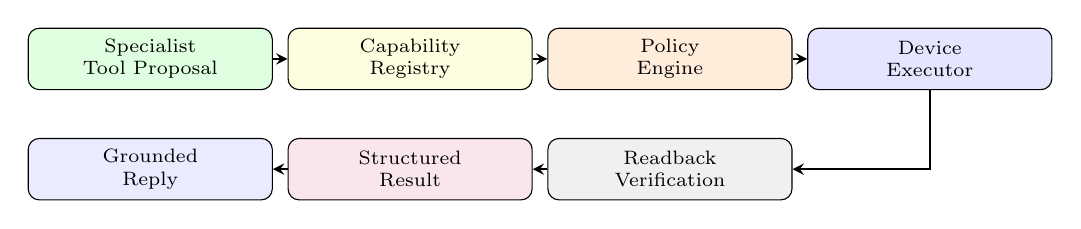
\begin{tikzpicture}[
            box/.style={draw, rounded corners, minimum width=3.1cm,
                    minimum height=0.78cm, align=center, font=\scriptsize},
            arrow/.style={->, >=stealth, thick}
        ]
        \node[box, fill=green!12] (plan) at (0,0) {Specialist\\Tool Proposal};
        \node[box, fill=yellow!12] (cap) at (3.3,0) {Capability\\Registry};
        \node[box, fill=orange!14] (policy) at (6.6,0) {Policy\\Engine};
        \node[box, fill=blue!10] (exec) at (9.9,0) {Device\\Executor};
        \node[box, fill=gray!12] (verify) at (6.6,-1.4) {Readback\\Verification};
        \node[box, fill=purple!10] (result) at (3.3,-1.4) {Structured\\Result};
        \node[box, fill=blue!8] (reply) at (0,-1.4) {Grounded\\Reply};

        \draw[arrow] (plan) -- (cap);
        \draw[arrow] (cap) -- (policy);
        \draw[arrow] (policy) -- (exec);
        \draw[arrow] (exec) |- (verify);
        \draw[arrow] (verify) -- (result);
        \draw[arrow] (result) -- (reply);
    \end{tikzpicture}
    \caption{Safe tool execution path for effectful device-control requests.}
    \label{fig:hera-safe-tool-path}
\end{figure}

\subsection{Memory and Discourse Grounding}

The graph maintains session state through a LangGraph checkpointer and optionally persists memory through MongoDB. H.E.R.A uses memory selectively rather than attaching all history to every request. This design avoids unnecessary context growth and reduces the chance that old conversation turns influence unrelated device commands. The system uses three practical memory concepts:

\begin{itemize}[leftmargin=*, itemsep=2pt]
    \item \textbf{Chat history} for coherent multi-turn conversation.
    \item \textbf{Recent actions} for resolving follow-up commands such as ``turn it off''.
    \item \textbf{Active focus} for carrying a currently discussed device target across turns.
\end{itemize}

The router chooses whether memory is needed. If memory scope is \texttt{none}, read-only requests can use the short path. If the request depends on prior context, the graph retrieves memory before selecting the specialist. This gives H.E.R.A contextual ability without making every request expensive or unpredictable.

\subsection{Model Provider and Current Configuration}

The LLM layer is provider-agnostic through LiteLLM. H.E.R.A currently supports two providers:

\begin{itemize}[leftmargin=*, itemsep=2pt]
    \item \textbf{Ollama:} local inference through \texttt{http://localhost:11434}, suitable for offline and privacy-sensitive operation.
    \item \textbf{OpenRouter:} cloud inference through the configured OpenRouter API base URL, suitable for flexible model access and easier deployment on machines without sufficient local GPU capacity.
\end{itemize}

The current runtime provider is \texttt{openrouter}. Model settings are loaded from MongoDB collection \texttt{model\_settings} using document id \texttt{hera\_model\_settings}; if that document is unavailable, H.E.R.A falls back to code-level defaults. In the current project run, the dashboard settings API reports the model assignments shown in Table~\ref{tab:hera-current-model-config}. The project environment file configures provider endpoints such as the Ollama API base URL and OpenRouter base URL, while model names are controlled by the runtime settings store.

\begin{table}[H]
    \centering
    \caption{Current configured model assignment in the H.E.R.A runtime}
    \label{tab:hera-current-model-config}
    \renewcommand{\arraystretch}{1.18}
    \begin{tabularx}{\textwidth}{@{}p{3.4cm}p{4.0cm}X@{}}
        \toprule
        \textbf{Role} & \textbf{Ollama configuration} & \textbf{OpenRouter configuration} \\
        \midrule
        Orchestrator router/composer & \path{gemma4:e4b} & \makecell[l]{\path{nvidia/nemotron-nano-}\\\path{9b-v2}} \\
        Device Control Agent & \makecell[l]{\path{TechyShishy/}\\\path{ministral-3:3b}} & \makecell[l]{\path{qwen/qwen3-30b-a3b-}\\\path{instruct-2507}} \\
        Sensor Analysis role & \makecell[l]{\path{TechyShishy/}\\\path{ministral-3:3b}} & \makecell[l]{\path{nvidia/nemotron-3-nano-}\\\path{omni-30b-a3b-reasoning:free}} \\
        Anomaly Expert role & \makecell[l]{\path{TechyShishy/}\\\path{ministral-3:3b}} & \makecell[l]{\path{nvidia/nemotron-3-nano-}\\\path{omni-30b-a3b-reasoning:free}} \\
        \bottomrule
    \end{tabularx}
\end{table}

Although the settings schema still contains sensor and anomaly model fields, the current telemetry and anomaly specialists are deterministic services. Their model fields remain useful for future LLM-based explanation upgrades, but the present implementation deliberately keeps core telemetry and anomaly classification outside the LLM.

\subsection{Model Selection Rationale}

The model configuration follows a cost-capability split. Routing benefits from a smaller model because the output space is bounded and latency matters. Device control uses a stronger instruction-following model because it must parse multilingual commands, room-level aliases, device values, conditional clauses, and clarification cases. The local Ollama configuration prioritizes offline availability with compact models, while the OpenRouter configuration assigns a larger Qwen model to device planning and Nemotron-family models to routing and explanatory roles. This split reflects the practical difference between low-cost local operation and cloud-assisted capability.

The OpenRouter-side selection was not based only on model popularity. H.E.R.A was tested with simple dashboard prompts before integration, and the NVIDIA response behavior was the most stable among the candidate responses observed in the local comparison. Figures~\ref{fig:hera-model-choose-1} and~\ref{fig:hera-model-choose-2} show these prompt-level checks. These checks are not treated as a formal benchmark; rather, they provide project-specific evidence that the selected model family follows the expected conversational style before being placed into a constrained orchestrator runtime.

\begin{figure}[H]
    \centering
    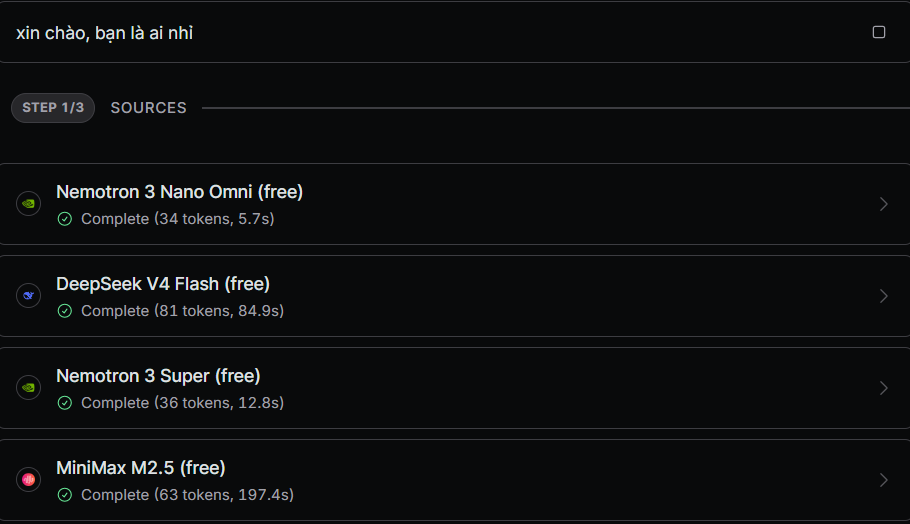
\includegraphics[width=0.92\textwidth]{image/system/model_choose1.png}
    \caption{Initial prompt-level comparison used during model selection.}
    \label{fig:hera-model-choose-1}
\end{figure}

\begin{figure}[H]
    \centering
    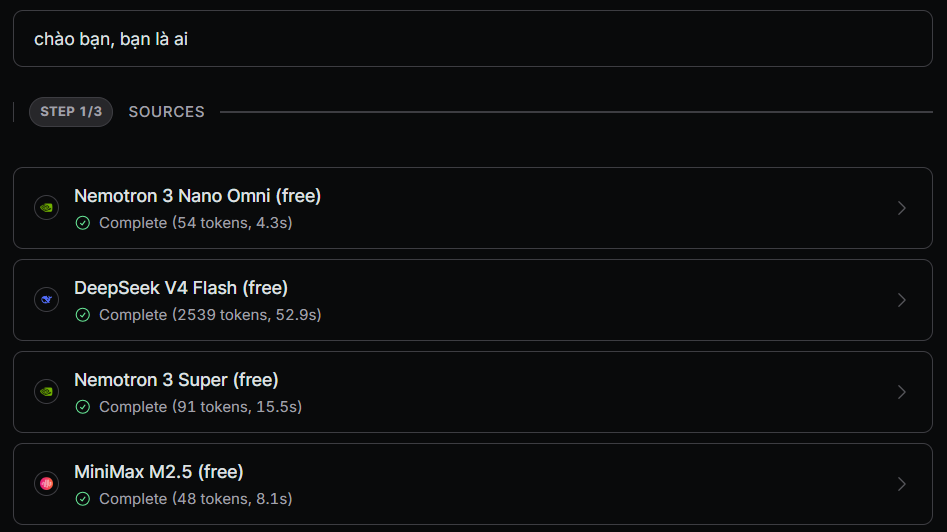
\includegraphics[width=0.92\textwidth]{image/system/model_choose2.png}
    \caption{Second prompt-level comparison used to validate response stability.}
    \label{fig:hera-model-choose-2}
\end{figure}

Because the H.E.R.A workload is specific to language understanding, intent routing, and tool-oriented execution, the model choice was also checked against public benchmark evidence. NVIDIA's model card for \texttt{NVIDIA-Nemotron-Nano-9B-v2} reports stronger results than Qwen3-8B on instruction following, coding/reasoning, long-context evaluation, and Berkeley Function Calling Leaderboard v3 (BFCL v3), a benchmark designed to evaluate function/tool-calling capability.\footnote{\url{https://huggingface.co/nvidia/NVIDIA-Nemotron-Nano-9B-v2}}\footnote{\url{https://sky.cs.berkeley.edu/project/berkeley-function-calling-leaderboard/}} The associated NVIDIA technical report further motivates the Nano-v2 family as an efficient hybrid Mamba-Transformer reasoning model, reporting comparable or better accuracy than similarly sized models with significantly higher inference throughput in long reasoning settings.\footnote{\url{https://arxiv.org/abs/2508.14444}} This external evidence matches the system-level requirement: the orchestrator model does not need to be the largest available model, but it must reliably follow instructions, preserve structured intent, and support agent/tool workflows.

\begin{table}[H]
    \centering
    \caption{External evidence used to justify the NVIDIA/Nemotron model family}
    \label{tab:hera-model-selection-evidence}
    \small
    \renewcommand{\arraystretch}{1.15}
    \begin{tabularx}{\textwidth}{@{}p{3.0cm}p{3.2cm}p{3.0cm}X@{}}
        \toprule
        \textbf{Evidence Source} & \textbf{Reported Metric} & \textbf{Reported Result} & \textbf{Relevance to H.E.R.A} \\
        \midrule
        NVIDIA model card & IFEval instruction strict & 90.3\% for Nemotron Nano 9B v2 vs. 89.4\% for Qwen3-8B & Supports the orchestrator role, where the model must follow routing and formatting instructions. \\
        NVIDIA model card & BFCL v3 tool calling & 66.9\% for Nemotron Nano 9B v2 vs. 66.3\% for Qwen3-8B & Directly relevant to tool-oriented agents because BFCL evaluates function/API calling accuracy. \\
        NVIDIA model card & RULER 128K long-context & 78.9\% for Nemotron Nano 9B v2 vs. 74.1\% for Qwen3-8B & Useful for multi-turn sessions where routing may depend on chat history, active focus, and recent actions. \\
        NVIDIA technical report & Efficiency claim & Up to 6$\times$ higher inference throughput in long reasoning settings compared with similarly sized models & Relevant to a dashboard assistant because lower perceived latency matters during repeated chat interactions. \\
        Project prompt checks & Simple user-facing prompts & NVIDIA responses were selected as the most stable in Figures~\ref{fig:hera-model-choose-1} and~\ref{fig:hera-model-choose-2} & Confirms that the public benchmark fit also appears in the project-specific conversational style. \\
        \bottomrule
    \end{tabularx}
\end{table}

\begin{table}[H]
    \centering
    \caption{Model role requirements for H.E.R.A}
    \label{tab:hera-model-role-requirements}
    \renewcommand{\arraystretch}{1.16}
    \begin{tabularx}{\textwidth}{@{}p{3.1cm}p{3.3cm}X@{}}
        \toprule
        \textbf{Role} & \textbf{Main requirement} & \textbf{Reason for model choice} \\
        \midrule
        Router & Structured intent classification & Small bounded output space; lower latency is more valuable than broad reasoning. \\
        Device planner & JSON command parsing and tool grounding & Requires stronger instruction following and robust handling of device aliases, values, and conditions. \\
        General response composer & Concise natural language & Needs fluent bilingual response generation but no direct tool access. \\
        Telemetry/anomaly services & Deterministic computation & Implemented without LLM decision-making to keep safety and evaluation auditable. \\
        Web research composer & Grounded summarization & Uses retrieved evidence but remains separated from actuator execution. \\
        \bottomrule
    \end{tabularx}
\end{table}

\subsection{Dashboard Streaming Mode}

The AI path described above still contains several latency sources: routing, model inference, specialist execution, optional tool execution, verification, and final response composition. Even when the backend completes correctly, returning the final answer as a single JSON payload makes the dashboard feel blocked until the full response is available. To reduce perceived latency, H.E.R.A introduces a streaming mode for the dashboard chat interface. This mode does not change the orchestrator's reasoning contract or the runtime tool boundary; it changes only how the already-generated assistant response is delivered to the frontend.

Streaming is enabled by adding the query parameter \texttt{stream=true} to the dashboard assistant endpoint. The backend endpoint \texttt{/api/assistant/message} first builds the same \texttt{UserMessage} object used by the non-streaming path and still calls the same orchestrator. After the orchestrator returns a structured response, the API server switches from a normal JSON response to a Server-Sent Events (SSE) stream. The SSE response uses \texttt{text/event-stream}, disables caching, keeps the connection open, and includes CORS headers so that the browser can consume the stream from the dashboard origin.

The backend streaming handler separates optional thinking metadata from final answer content. Thinking text, when present, is emitted in small three-character chunks with a short delay. Final answer text is emitted one character at a time with an approximately 20 ms delay, which produces a readable character-by-character response in the browser. Each message follows an OpenAI-compatible delta shape, such as \texttt{\{"choices":[\{"delta":\{"content":"H"\}\}]\}}, and the stream terminates with \texttt{data: [DONE]}. If the orchestrator fails before streaming begins, the backend returns the same error information through an SSE error payload so the frontend can surface the failure consistently.

On the frontend, \texttt{sendAssistantMessageStreaming()} in the dashboard API service sends the request with \texttt{stream=true}, attaches an \texttt{AbortSignal}, reads \texttt{response.body.getReader()}, decodes complete SSE lines, and accumulates content and thinking streams separately. The chat component creates an empty assistant placeholder before the first chunk arrives, tracks the active streaming message id with a React ref, and updates only that message as chunks arrive. This design avoids re-rendering unrelated chat history on every token. Where available, \texttt{ReactDOM.flushSync()} is used to force immediate rendering per chunk, preventing React batching from collapsing many chunk updates into one visual update.

\begin{table}[H]
    \centering
    \caption{Streaming-mode design decisions in the H.E.R.A dashboard chat}
    \label{tab:hera-streaming-design}
    \small
    \renewcommand{\arraystretch}{1.15}
    \begin{tabularx}{\textwidth}{@{}p{2.7cm}X X@{}}
        \toprule
        \textbf{Layer} & \textbf{Implementation Decision} & \textbf{Design Rationale} \\
        \midrule
        Backend API & The \texttt{/api/assistant/message} endpoint selects SSE delivery when \texttt{stream=true} after normal orchestrator execution & Preserves the existing AI control flow while changing only the delivery mode. \\
        Transport & SSE chunks use \texttt{data: ...} lines and terminate with \texttt{[DONE]} & Simple browser-native unidirectional streaming fits assistant responses without requiring WebSocket state. \\
        Chunking & Thinking chunks use three characters; answer chunks use one character with a 20 ms delay & Makes response progress visible and readable instead of appearing as a buffered block. \\
        Frontend parser & \texttt{ReadableStream} reader parses SSE lines and accumulates full text & Supports progressive rendering while still retaining the complete final answer for chat history. \\
        React state & Active message id is stored in a ref and updated directly through an indexed message update & Reduces per-chunk state work and avoids unnecessary updates to previous messages. \\
        User control & \texttt{AbortController} backs the pause action & Closing the fetch stream stops frontend updates and prevents wasted backend/network work. \\
        Fallback & If streaming returns JSON or fails, the frontend falls back to the non-streaming API path & Keeps the dashboard usable even when streaming is unsupported or interrupted. \\
        \bottomrule
    \end{tabularx}
\end{table}

This streaming design is therefore a presentation and responsiveness optimization, not a shortcut around safety. Tool execution still completes inside the runtime boundary before the final answer is streamed. The user receives the answer progressively, but the content remains grounded in the same verified orchestrator result as the non-streaming mode. This keeps the system design consistent with the rest of the H.E.R.A AI architecture: semantic reasoning and physical action remain controlled by the orchestrator and runtime layers, while the dashboard optimizes the delivery of the final user-facing response.

\subsection{End-to-End Device-Control Flow}

Figure~\ref{fig:hera-device-control-sequence} traces a representative command such as ``turn on the living room light''. The important point is that the LLM does not publish MQTT directly. It only proposes a structured action. The runtime validates and executes it.

\begin{figure}[H]
    \centering
    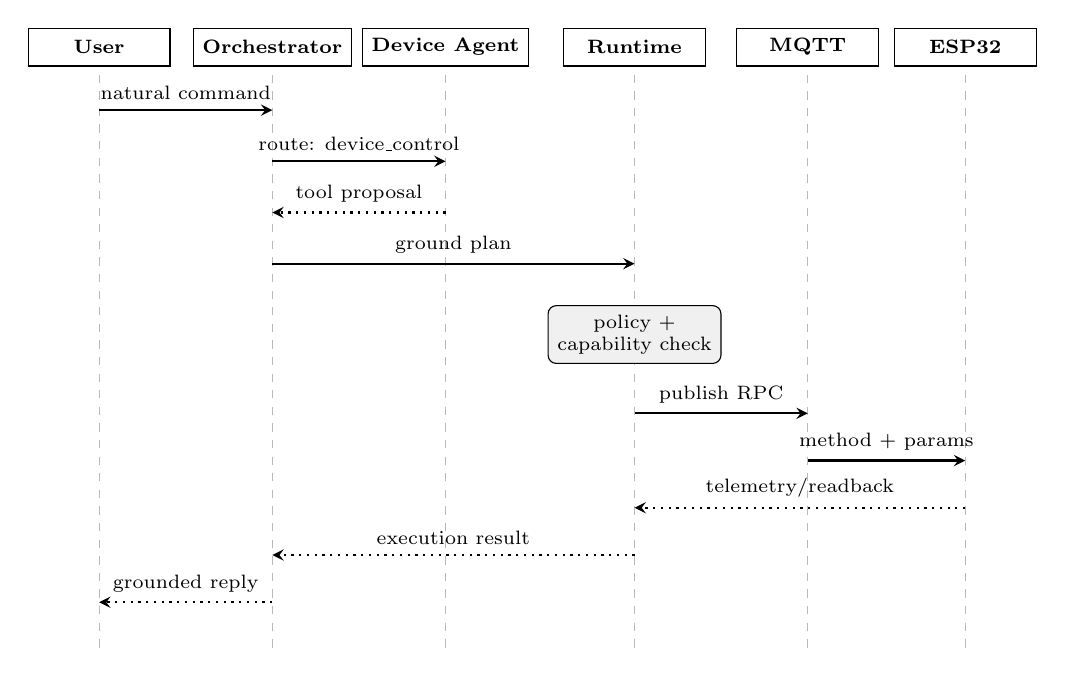
\begin{tikzpicture}[
            actor/.style={draw, rectangle, minimum width=1.8cm,
                    minimum height=0.48cm, align=center, font=\scriptsize\bfseries},
            msg/.style={->, >=stealth, thick},
            ret/.style={->, >=stealth, thick, dotted},
            internal/.style={draw, rounded corners=3pt, fill=gray!12,
                    minimum width=2.0cm, minimum height=0.48cm,
                    align=center, font=\scriptsize},
            lab/.style={font=\scriptsize, align=center}
        ]
        \def\u{0}
        \def\o{2.2}
        \def\d{4.4}
        \def\r{6.8}
        \def\m{9.0}
        \def\e{11.0}

        \node[actor] at (\u,0) {User};
        \node[actor] at (\o,0) {Orchestrator};
        \node[actor] at (\d,0) {Device Agent};
        \node[actor] at (\r,0) {Runtime};
        \node[actor] at (\m,0) {MQTT};
        \node[actor] at (\e,0) {ESP32};

        \foreach \x in {\u,\o,\d,\r,\m,\e} {
            \draw[dashed, gray!55] (\x,-0.35) -- (\x,-7.7);
        }

        \draw[msg] (\u,-0.8) -- node[above, lab] {natural command} (\o,-0.8);
        \draw[msg] (\o,-1.45) -- node[above, lab] {route: device\_control} (\d,-1.45);
        \draw[ret] (\d,-2.1) -- node[above, lab] {tool proposal} (\o,-2.1);
        \draw[msg] (\o,-2.75) -- node[above, lab] {ground plan} (\r,-2.75);
        \node[internal] at (\r,-3.65) {policy +\\capability check};
        \draw[msg] (\r,-4.65) -- node[above, lab] {publish RPC} (\m,-4.65);
        \draw[msg] (\m,-5.25) -- node[above, lab] {method + params} (\e,-5.25);
        \draw[ret] (\e,-5.85) -- node[above, lab] {telemetry/readback} (\r,-5.85);
        \draw[ret] (\r,-6.45) -- node[above, lab] {execution result} (\o,-6.45);
        \draw[ret] (\o,-7.05) -- node[above, lab] {grounded reply} (\u,-7.05);
    \end{tikzpicture}
    \caption{End-to-end sequence for a device-control request.}
    \label{fig:hera-device-control-sequence}
\end{figure}
